%%%%%%%%%%%%%%%%%%%%%%%%%%%%%%%%%%%%%%%%%%%%%%%%%%%%%%%%%%%%%%%%%%%%%%%%%%%%%%%%
%2345678901234567890123456789012345678901234567890123456789012345678901234567890
%        1         2         3         4         5         6         7         8

\documentclass[letterpaper, 10 pt, conference]{ieeeconf}  % Comment this line out if you need a4paper

%\documentclass[a4paper, 10pt, conference]{ieeeconf}      % Use this line for a4 paper

\IEEEoverridecommandlockouts                              % This command is only needed if 
% you want to use the \thanks command

\overrideIEEEmargins                                      % Needed to meet printer requirements.

%In case you encounter the following error:
%Error 1010 The PDF file may be corrupt (unable to open PDF file) OR
%Error 1000 An error occurred while parsing a contents stream. Unable to analyze the PDF file.
%This is a known problem with pdfLaTeX conversion filter. The file cannot be opened with acrobat reader
%Please use one of the alternatives below to circumvent this error by uncommenting one or the other
%\pdfobjcompresslevel=0
%\pdfminorversion=4

% See the \addtolength command later in the file to balance the column lengths
% on the last page of the document

% The following packages can be found on http:\\www.ctan.org
\usepackage{graphics} % for pdf, bitmapped graphics files
\usepackage{epsfig} % for postscript graphics files
%\usepackage{mathptmx} % assumes new font selection scheme installed
%\usepackage{times} % assumes new font selection scheme installed
\usepackage{amsmath}
\usepackage{amssymb}  % assumes amsmath package installed
%\usepackage[hidelinks]{hyperref}
\usepackage{hyperref}
\usepackage{subcaption}
%\usepackage{array}
\usepackage[table]{xcolor}
\usepackage{collcell}
\usepackage{hhline}
\usepackage{pgf}
\usepackage{pgfplots}
\usepackage{multirow}
\usepackage[ruled,vlined]{algorithm2e}
\usepackage{booktabs,dcolumn}
\usepackage{etoolbox,siunitx}
\captionsetup{labelsep=newline,
	singlelinecheck=false,
	skip=0.333\baselineskip}

\title{\LARGE \bf
	Coverage Path Planning in Large-scale Multi-floor Urban Environments with Applications to Autonomous Road Sweeping
}


\author{Daniel Engelson$^{1}$ and Mattias Tiger$^{1}$ and Fredrik Heintz$^{1}$% <-this % stops a space
	\thanks{*This work was not supported by any organization}% <-this % stops a space
	\thanks{$^{1}$Danil Engelson, Mattias Tiger and Fredrik Heintz are with the Department of Computer and Information Science, Link{\"o}ping University, Sweden.
		{\tt\small mattias.tiger@liu.se, fredrik.heintz@liu.se}
	}%
}


\begin{document}
	
	
	
	\maketitle
	\thispagestyle{empty}
	\pagestyle{empty}
	
	
	%%%%%%%%%%%%%%%%%%%%%%%%%%%%%%%%%%%%%%%%%%%%%%%%%%%%%%%%%%%%%%%%%%%%%%%%%%%%%%%%
	\begin{abstract}
		
		
	\end{abstract}
	
	
	%%%%%%%%%%%%%%%%%%%%%%%%%%%%%%%%%%%%%%%%%%%%%%%%%%%%%%%%%%%%%%%%%%%%%%%%%%%%%%%%
	\section{INTRODUCTION}
	Enterprise and household robots routinely perform simple service tasks, with a demand for better performance, less maintenance and a wider set of tasks growing steadily \cite{frey2017future}. Many of the most well-recognized automated service tasks today such as \emph{lawn moving}, \emph{vacuuming} and \emph{mopping} are powered by algorithms performing \emph{Coverage Path Planning} (CPP) \cite{galceran2013survey}. The CPP task is to generate a path that covers a map while avoiding obstacles. Steady progress has been made both regarding faster planners which generates better (e.g. short) paths and wider applicability \cite{bormann2018indoor}. 
	CPP can be divided into two types, the \emph{Sensor Coverage Problem} and the \emph{Footprint Coverage Problem} \cite{bormann2018indoor}. Examples of the former is \emph{3D exploration} \cite{schmid2020efficient}, where a sensor has to be placed at sufficient poses as to fully capture a map. Examples of the latter is \emph{floor cleaning} \cite{bormann2015new}, where it is the robot, or its actuator, that has to be placed to cover the entire map. The Footprint Coverage Problem type of CPP is the focus here.
	
	The CPP problem can be solved using A* search but it is intractable to solve to optimum for even small toy problems \cite{dogru2017based}. The reason for this is that CPP is NP-hard \cite{arkin2000approximation} and therefore necessitate approximate or heuristic algorithms for solving CPP problems in practice. Algorithms have been developed that are tailored to specific application contexts, leveraging the specific circumstances such as flat surfaces on single floors or rigid shapes and small scales permitting efficient use of grid representations. These are common characteristics of most indoor environment and outdoor lawns.
	
	%TODO? Previous work has considered large-scale but "simple" world. Or small-scale cluttered worlds. Or indoor worlds easily divided into rooms or rectangular regions.
	
	In this paper we consider offline CPP in the context of real-world \emph{urban environments}. Such outdoor environments are characterized by a combination of large scales and complex surface geometry, with challenging aspects including non-flat surfaces, being partially cluttered and possibly multi-floor. A natural division between distinct rooms or floors are lacking, in contrast with general indoor environments studied in most of the literature \cite{galceran2013survey,bormann2018indoor}. The surface geometry also differs from the characteristic regular straight lines and rectangular rooms of the indoor setting \cite{bormann2018indoor}, and of the non-cluttered, rigid or smooth geometry of outdoor setting in agriculture such as croplands \cite{oksanen2009coverage,hameed2016side} and customary lawns \cite{einecke2018boundary}. 
	
	Real 3D environments are captured using LIDAR or 3D-sensors as point clouds. Further discretization can be made, for example using Octomap \cite{octomap}, but there are several benefits with working directly on a point cloud. Good coverage can be achieved while avoiding an intractably high voxel resolution, given that the point cloud distribution is fairly even over surfaces and that the point density is kept down to manageable levels. Furthermore, while planar or voxel-based surface approximations can be efficient representations, motion planning on such approximations may lead to unfeasible plans. A plan that seemed to be the shortest of all explored alternatives can be impossible to follow, lead to unsafe execution or be worse (e.g. take longer to follow) than other plans which seem worse during planning \cite{krusi2017driving}.
	%TODO: Also, motion planning on point clouds: \cite{krusi2017driving}. They have motivations, eh?
	
	
	%TODO: Right column
	\begin{figure}[t]
		\centering
		\begin{subfigure}{\columnwidth}
			\centering
			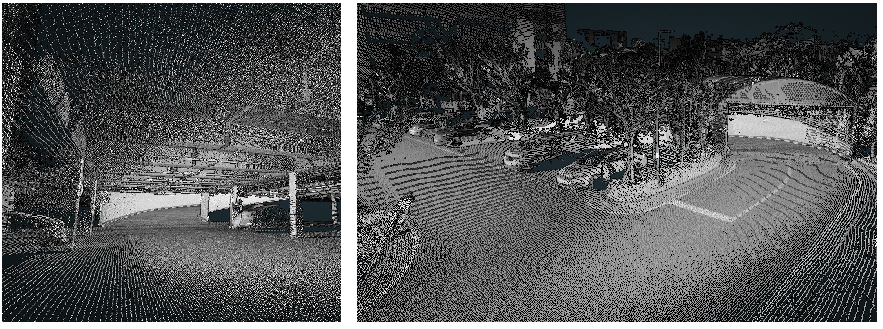
\includegraphics[width=\textwidth]{figures/environment.pdf}
		\end{subfigure}
		\begin{subfigure}{\columnwidth}
			\centering
			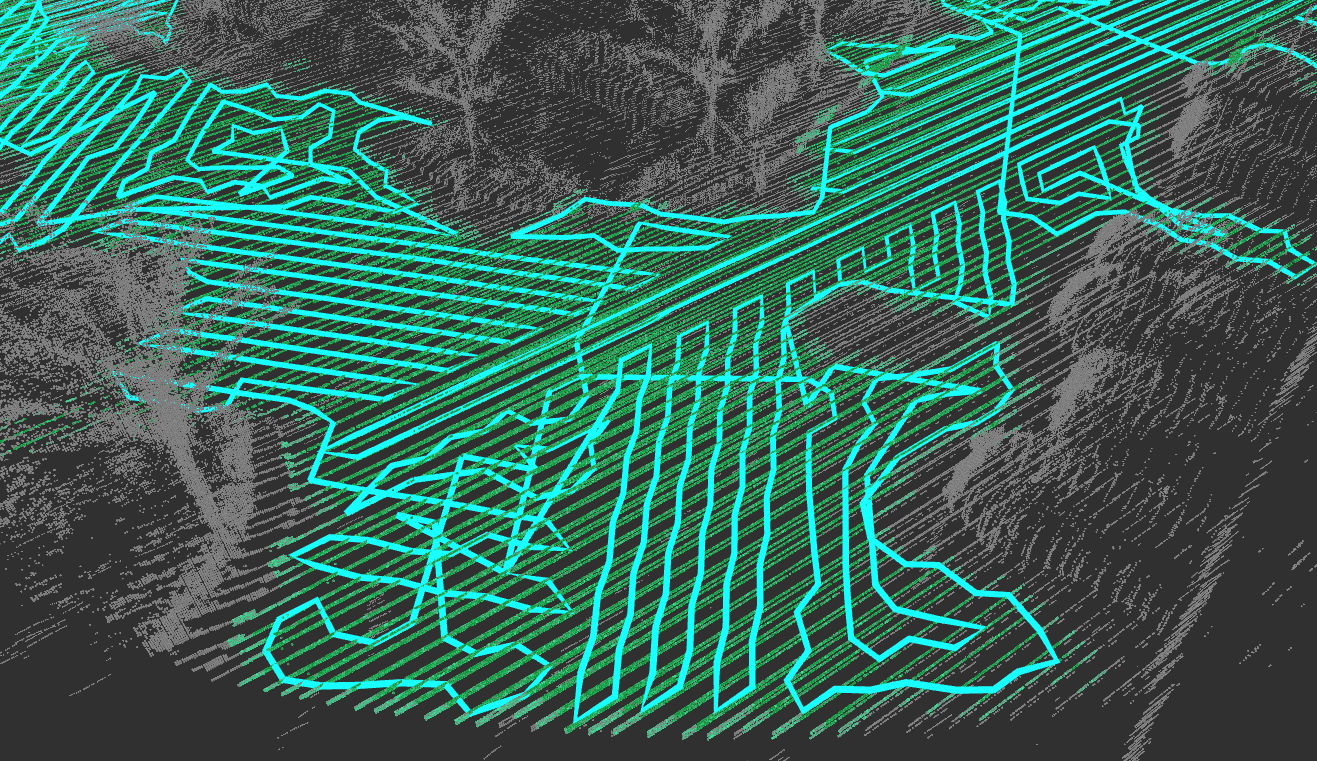
\includegraphics[width=\textwidth]{figures/example_sampled_bastar.png}
		\end{subfigure}
		\caption{\textbf{Top:} Garage point cloud. \\\textbf{Bottom:} Covering path from our approach.}
		\label{fig:example}
	\end{figure}
	
	The task investigated in this paper is that of CPP for autonomous road sweeping (Figure \ref{fig:example}), where the input is a point cloud and the output is a collision free path with highest possible coverage while minimizing path length and total rotation.
	%TODO (related work?): Previous work \cite{bormann2018indoor} (and their previous work) map indoor environment and has pipeline for automatic segmentation of map into single rooms and TSP for efficient visitation between rooms.	
	The main contributions of this paper are:
	\begin{itemize}
		\item A benchmark suite\footnote{Code and benchmark suite will be made publicly available upon paper acceptance.} consisting of three large-scale urban environments as point clouds, with and without labeled points. They span a variety of multi-floor and complex geometry, representative of outdoor road sweeping tasks under difficult and varying real-world conditions.
		\item Evaluation of prominent CPP algorithms on the urban outdoor CPP task.
		\item A proposed CPP algorithm that out-performs state-of-the-art CPP algorithms at this task.
		\item Parameter optimization of CPP algorithms for automatic domain adaptation, for evaluation and as part of an enhanced offline meta-CPP algorithm.
	\end{itemize}
	
	The outline is as follows. In section \ref{sec:problem} the problem is formally summarized, in section \ref{sec:related-work} related work is discussed and relevant background material is presented in \ref{sec:background}. Section \ref{sec:terrain-assessment} describe how 3D point clouds are analyzed to determine the sets of points traversable and coverable by the robot. The proposed CPP algorithm is detailed in section \ref{sec:proposed-method}, and the benchmark suite including, three 3D point clouds representative for the urban road sweeping task, is presented in \ref{sec:scenario-environment}. Section \ref{sec:evaluation} contains the evaluation of CPP algorithms on the benchmark and section \ref{sec:conclusions} concludes the paper.
	
	\section{Problem Formulation}
	\label{sec:problem}
	%TODO: Heading angle (or full 6-DOF?)
	Consider a robot with geometry $R\subset \mathbb{R}^3$ that can travel over a surface with a maximum height difference of $h^R_{max}$.
	Given a bounded 3D world $\mathcal{W}\in\mathbb{R}^3$ and a starting point $x_S$, the set $\mathcal{W}_{cov}\subseteq \mathcal{W}$ contain all surface points that the are coverable by the robot. A surface point $p$ is coverable by the robot if there is a point $x\in\mathcal{W}$ for which the robot placed at $x$ cover $p$ with its geometry $R$, and if $x$ is reachable from $x_S$ for the robot without collisions.
	
	The Coverage Path Planning (CPP) problem is to find a path $P$ of states $x\in P$ such that every point $p\in\mathcal{W}_{cov}$ must have been inside $R$ at least once when placing $R$ at every position in $P$. 
	
	The task is to determine $\mathcal{W}_{cov}$ and subsequent a path starting in $x_S$ that let the robot cover all coverable points $x\in\mathcal{W}_{cov}$ while minimizing the path cost.
	
	\section{Related Work}
	\label{sec:related-work}
	\begin{itemize}
		\item Indoor coverage path planning
		\item Outdoor coverage path planning
		\item 3D exploration (Sensor Coverage Problem vs Foot print Coverage Problem)
		\item Online coverage path planning
	\end{itemize}
	
	Our problem formulation differs from related work. The sets of traversable and coverable points are not the same set. We operate on a point cloud, not on a grid or explicit cells (although we have implicit cells?). We must determine which points (regions) that are traversable and coverable. The environment under consideration can be multi-floor but is outdoor (\cite{terrainassessment} is multi-floor terrain assessment in small confined indoor settings. Their related work is conserned with larger outdoor but single-floor terrain assessment. Note: old papers..).
	
	Large indoor environments (grid size of 1000x1000) are considered by \cite{miao2018scalable} such as a library, a gym, an airport. They show that BA* generates best local paths, but long paths between local regions. They propose a method that is better than BA* on the total path length. Seem to generate more rotations though..? (We might need to motivate why we didn't compare with their proposed approach)
	
	\section{Background}
	\label{sec:background}
	\begin{itemize}
		\item BA* \cite{viet2013ba}
		\item Inward Spiral \cite{zhang2019path}
		\item Sampling-Based Sweep Planning \cite{englot2012sampling}
		\item TSP\dots(?)
	\end{itemize}
	
	\subsection{BA*}
	BA* \cite{viet2013ba} is based on Boustrephedon motions \cite{choset1998coverage} and the A* search algorithm \cite{russell_artificial_2020}. The algorithm consists of following steps:
	\begin{enumerate}
		\item Cover the local area using the Boustrophedon motion (BM) algorithm until a critical point is reached and no further Boustrophedon motion is possible.
		\item Use a backtracking list to find the next starting point.
		\item Use A* to plan a collision free path to the next starting point.
		\item Shorten the path using the A*SPT \cite{viet2013ba} algorithm.
		\item Follow the generated path and go to step 1 to cover a new area.
	\end{enumerate}
	These steps are repeated until Step 2 can no longer find a new uncovered starting point.
	
	\subsection{Inward Spiral}
	Inward Spiral \cite{zhang2019path} works by counter-clockwise motion. The algoritm consists of the following steps:
	\begin{enumerate}
		\item Clean area in an inward spiral motion until a dead zone is reached
		\item Find closest uncovered accessible point using Breadth-first search \cite{russell_artificial_2020}.
		\item Find shortest path using A* to the closest uncovered point and go back to Step 1.
	\end{enumerate}
	This cycle repeats until the area has been covered.
	
	\subsection{Sampling-Based Coverage Path Planning}
	?
	
	\subsection{Strength and Weaknesses}
	\dots
	
	%TODO: Reference to A$^*$: \cite{russell_artificial_2020}
	
	\section{Terrain Assessment}
	\label{sec:terrain-assessment}
	Multi-floor indoor \cite{terrainassessment}?
	
	\begin{figure}
		\centering
		\begin{subfigure}{.49\columnwidth}
			\centering
			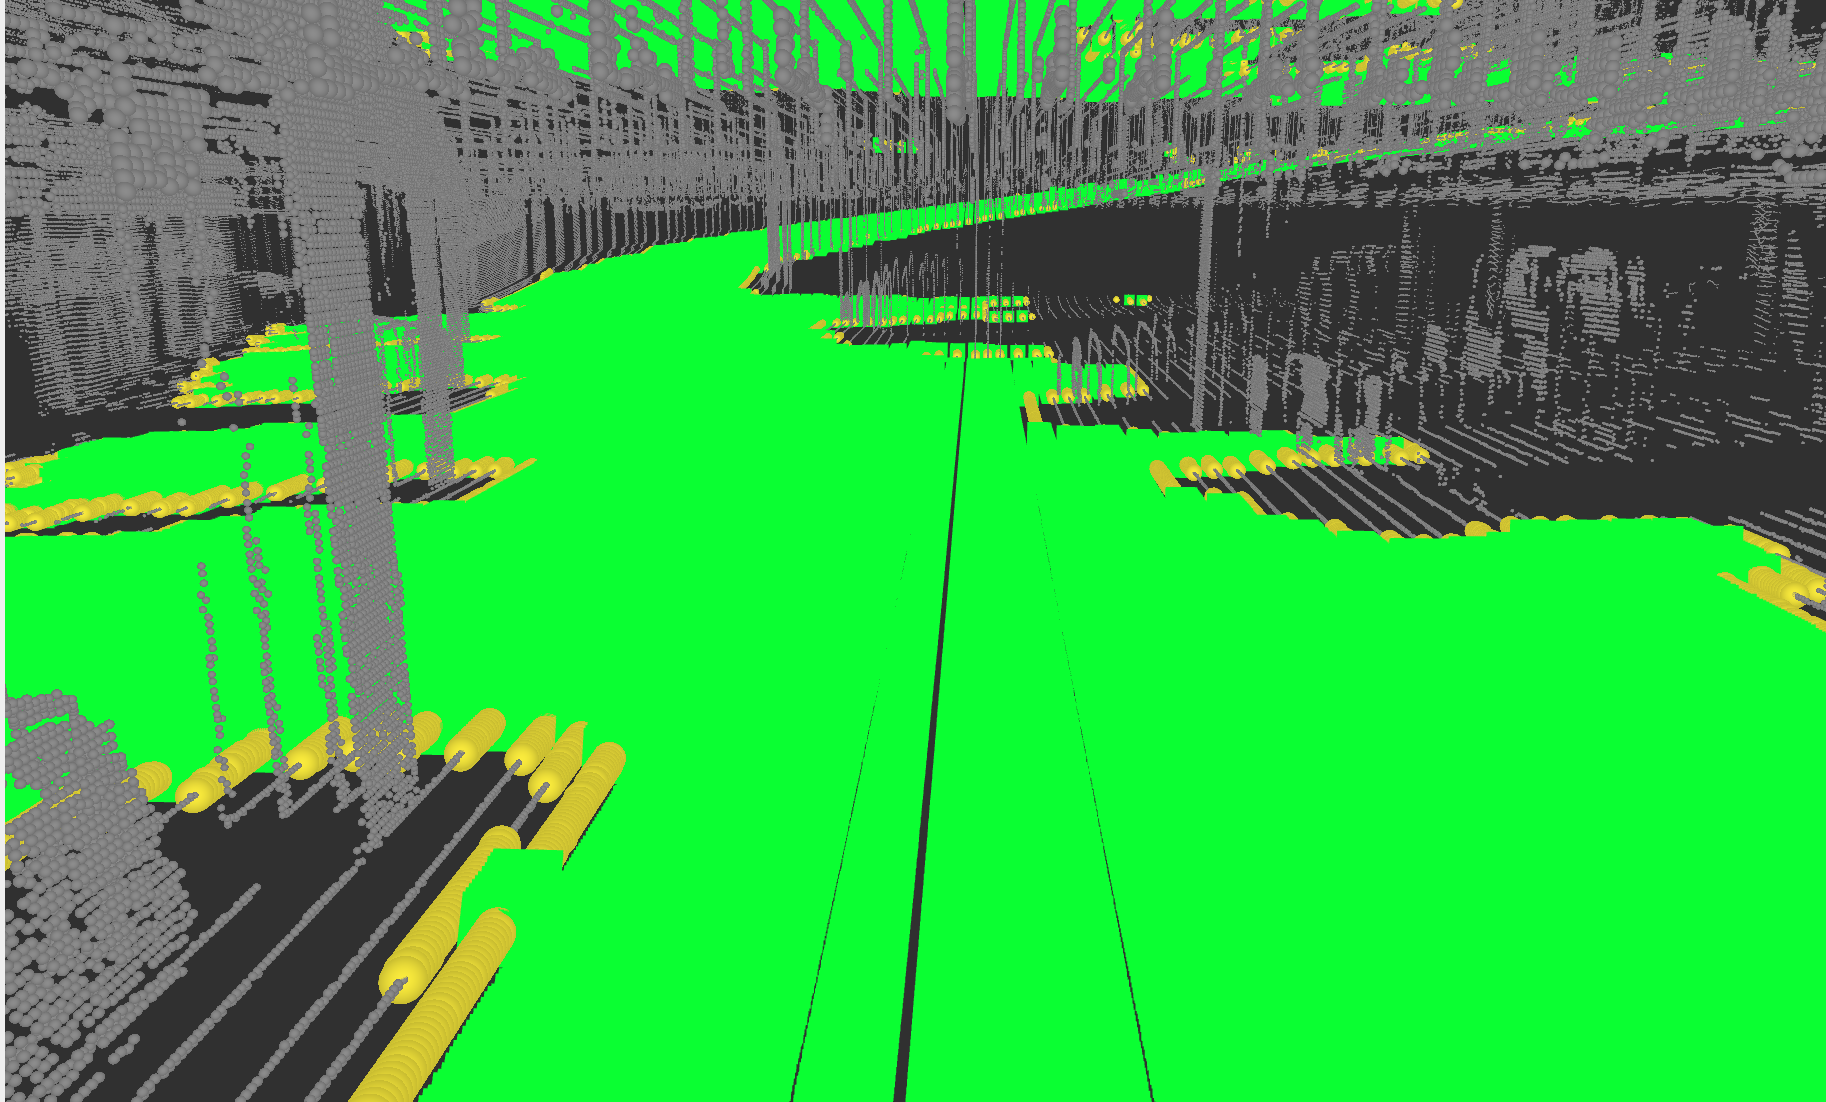
\includegraphics[width=\textwidth]{figures/terrainassessment-floor1.png}
			\caption{Viewed from Floor 1}
		\end{subfigure}
		\begin{subfigure}{.49\columnwidth}
			\centering
			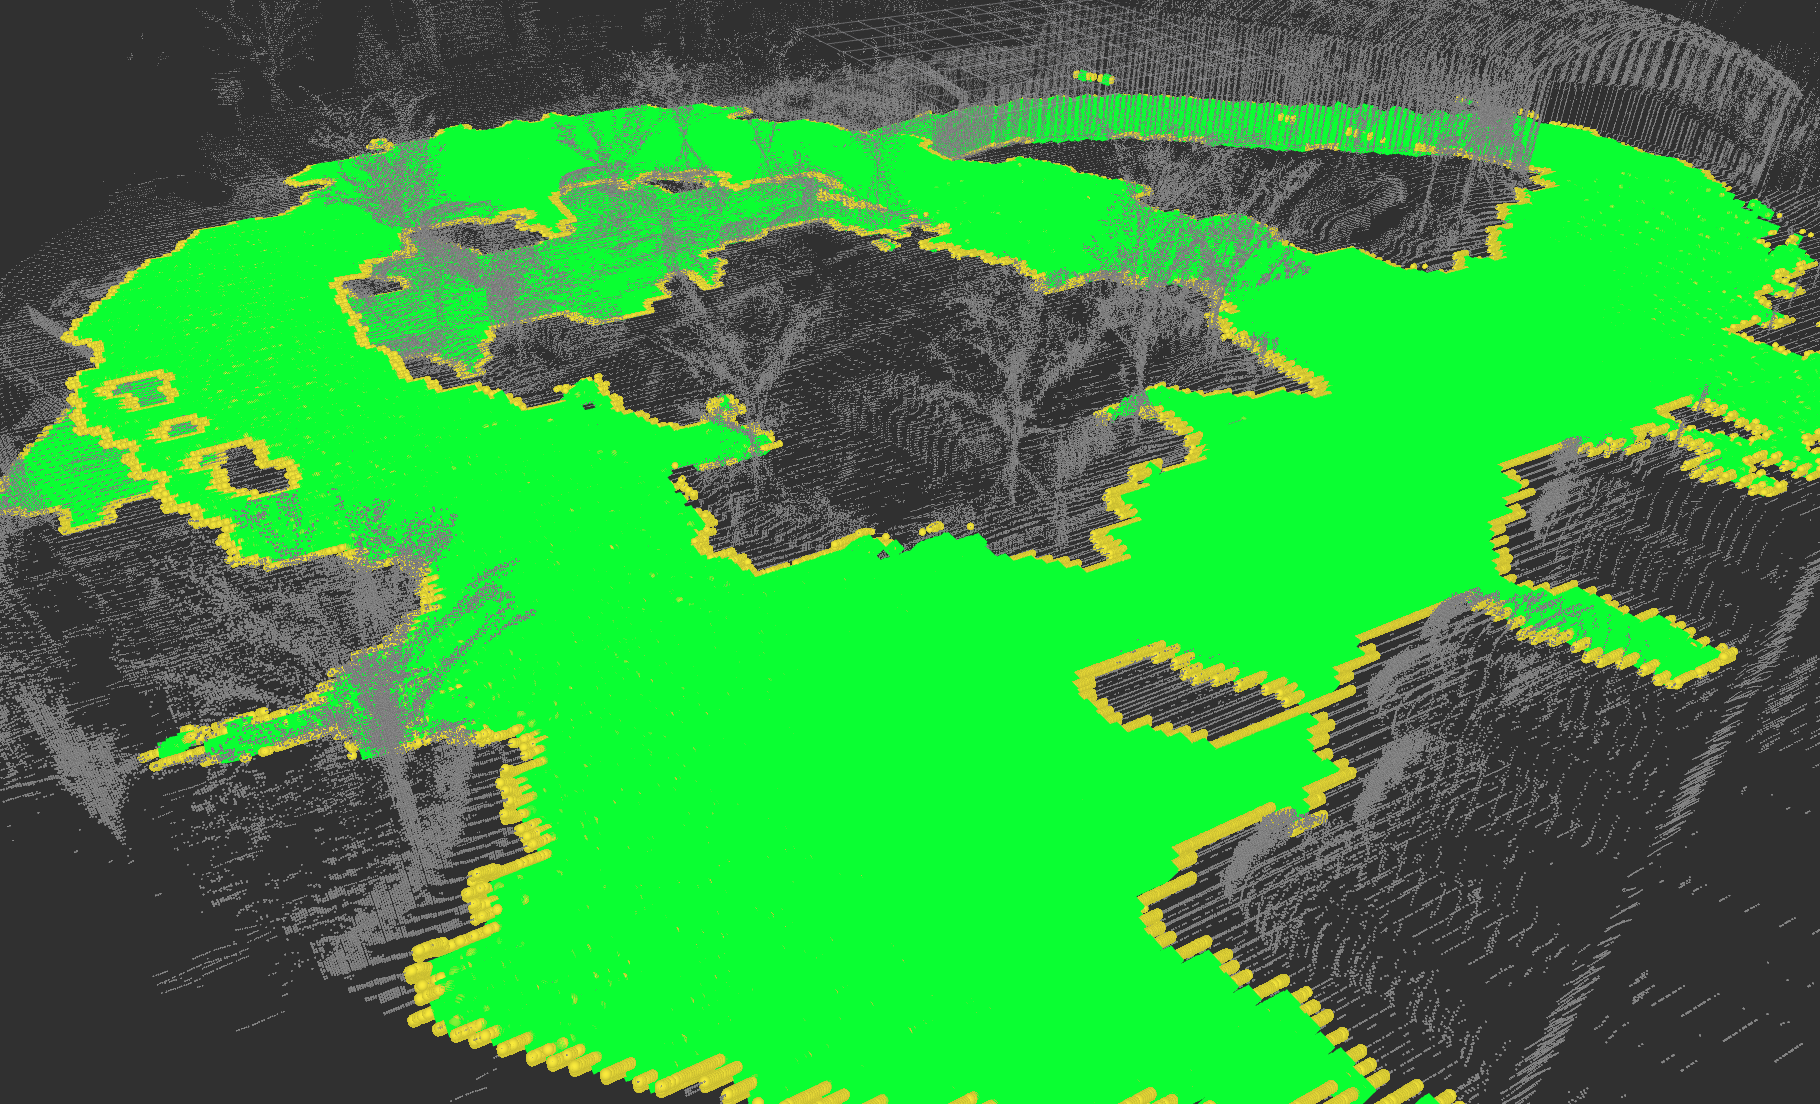
\includegraphics[width=\textwidth]{figures/terrainassessment-floor2.png}
			\caption{Viewed from Floor 2}		
		\end{subfigure}	
		\caption{Result of Terrain Assessment on Garage. Green points represents traversable areas, yellow are only coverable and grey are points that are obstacle and inaccessible points}
		\label{fig:terrainassessment}
	\end{figure}
	
	\section{Proposed Method (sBA*-Spiral-TSP)}
	\label{sec:proposed-method}
	\textit{Sample-Based BA* and Inward Spiral with Traveling Salesman} (SBA*SITSP)\dots
	
	An approach that combines the strengths of BA* \cite{viet2013ba}, Inward Spiral \cite{zhang2019path} and Sampling-Based Sweep Planning \cite{englot2012sampling}\dots
	
	The idea is to cover open areas with BA* and more complex areas with Inward Spiral. This is done by covering segments of the area with BA* and Inward Spiral starting from random sampled points and then connect these segments with a TSP solver. The new algorithm, see \ref{alg:myalgorithm}, follows these steps:
	
	\begin{enumerate}
		\item Use random sampling to get an unvisited \emph{Traversable} point $p_s$.
		\item For $N_\phi$ different angles $\phi_i$, define $north$ as the angle $\phi_i$ and start covering using the BA* algorithm \cite{viet2013ba} starting from starting point $p_s$. Keep covering until the distance to the next starting point, generated by CPP Step 2, is bigger than a hand tuned threshold, $d_{max}$. See illustration in Figure \ref{fig:myalga}.
		\item Step 2 will generate $N_\phi$ different paths from the same starting point $p_s$. Pick the path that covers the biggest area and add it to a list with paths that covers different segments, $S$.
		\item Repeat the Step 1-3 until a pre defined coverage percentage, $C_1$ or a maximum amount of iterations $N^{iter}_{max}$ has been reached.
		\item Use random sampling to get an unvisited \emph{Traversable} point $p_s$.
		\item Start covering using the Inward Spiral algorithm \cite{zhang2019path} starting from starting point $p_s$, see Figure \ref{fig:myalgb}. Keep covering until the distance to the next starting point, generated by CPP Step 2, is bigger than a hand tuned threshold, $d_{max}$. Add the path to $S$.
		\item Repeat the Step 5-6 until a pre-defined coverage percentage, $C_2$ has been reached.
		\item Build up a graph tree, $T$, from $S$. Only the start and end positions of the paths in $S$ are added as nodes to $T$. All nodes are connected with edges with weights set to 
		\begin{itemize}
			\item $w=0$, if the edge is between the start and end node of the same path in $S$.
			\item Otherwise, distance based  according to equation 
			\begin{align}
			\label{eq:distanebased}
			w = \;&w_\text{offset} + \\
			& | s_A(x,y) - s_B(x,y) | + \nonumber\\
			&K | s_A(z) - s_B(z) |\nonumber
			\end{align}
			where $s_A$ and $s_B$ are the position of the two nodes, $w_\text{offset}$ is a large number and $K\geq 1$.
		\end{itemize}
		
		The purpose of $w_\text{offset}$ is to make sure that the traveling salesman algorithm in the following step always chooses to connect corresponding start and end nodes. Since the environment had multiple floors extra weight is added to difference in height, since the path in most cases will be longer. This is the purpose of coefficent $K$.
		\item Apply a traveling salesman algorithm to calculate the cheapest route, $W_\text{TSP}$, to visit all nodes in $T$, see Figure \ref{fig:myalgc}. An approximate local search TSP algorithm \cite{python-tsp} was used.
		\item Walk through every node in $W_\text{TSP}$ and create a ordered list of paths $S_\text{TSP}$. For every node $s_i$,
		\begin{itemize}
			\item If $s_i$ is a start node, add the corresponding path in $S$ to $S_\text{TSP}$.
			\item If $s_i$ is a end node, add the corresponding path, but reversed, in $S$ to $S_\text{TSP}$.
		\end{itemize}
		\item Create a continuous path $W$ by following the paths in $S_\text{TSP}$. Connect them with obstacle free smooth A* paths, as in CPP Step 3 in previous CPP implementations. See illustration in Figure \ref{fig:myalgd}.
	\end{enumerate}
	
	%\newpage
	%\newpage
	%\begin{figure}
	%	\centering
	%	\begin{subfigure}{\columnwidth}
	%		\centering
	%		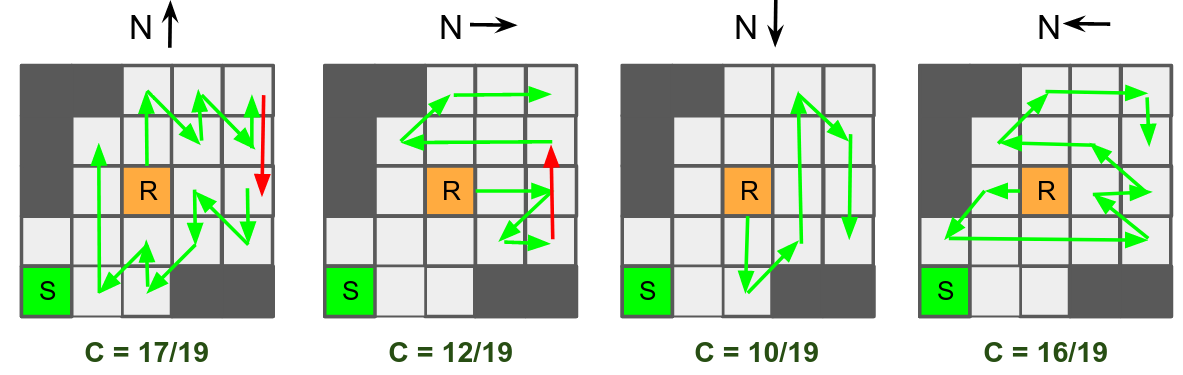
\includegraphics[width=\textwidth]{figures/Sampled_BA.png}
	%		\caption{For different angles $\phi_i$, define north $N$ as the angle $\phi_i$ and start covering using the BA* starting from random sampled point $R$. Keep covering until the distance to the next starting point is too big. Choose the path with the biggest coverage $C$.}
	%		\label{fig:myalga}
	%	\end{subfigure}
	%	\\
	%	\begin{subfigure}{0.5\columnwidth}
	%		\centering
	%		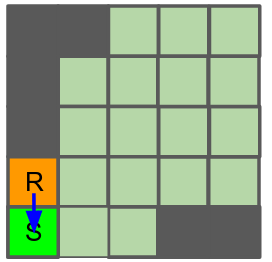
\includegraphics[width=1\textwidth]{figures/Sampled_inward.png}
	%		\caption{Start covering using the Inward Spiral algorithm starting from random sampled uncovered point $R$. Green boxes in the figure are covered by the BA*. See the first path from left in Figure \ref{fig:myalga}.}
	%		\label{fig:myalgb}
	%	\end{subfigure}
	%	\\
	%	\begin{subfigure}{\columnwidth}
	%		\centering
	%		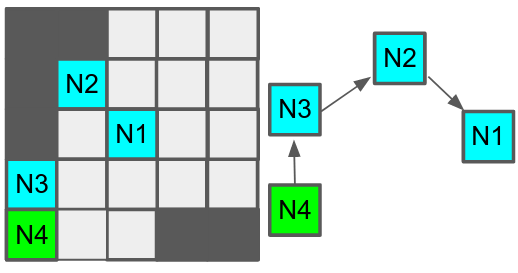
\includegraphics[width=1\textwidth]{figures/Sampled_TSP.png}
	%		\caption{Apply a traveling salesman algorithm to calculate the cheapest route to visit all start and end points of path. Since the weight between start and end node pairs is set to 0 they will always be connected. In this case, the TSP could have chosen the edge $N3\rightarrow N1$ as well since the cost is the same as $N3\rightarrow N2$. The latter was chosen to demonstrate that the path get reversed, see Figure \ref{fig:myalgd}, since $N2$ is an end node.}
	%		\label{fig:myalgc}
	%	\end{subfigure}
	%	\\
	%	\begin{subfigure}{0.5\columnwidth}
	%		\centering
	%		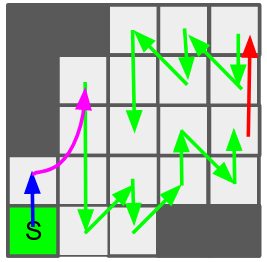
\includegraphics[width=1\textwidth]{figures/Sampled_total.png}
	%		\caption{The final path. The robot follows all paths according to the cheapest route and connects them using smooth A*, see purple arrow. Since $N2\rightarrow N1$ starts from and end node, the path is reversed to the path in \ref{fig:myalga}}
	%		\label{fig:myalgd}
	%	\end{subfigure}
	%	
	%	\caption{Simplified illustration of the Sampling-based BA* and Inward Spiral with Traveling Salesman algorithm.}
	%	\label{fig:myalg}
	%\end{figure}
	%\newpage
	


%\begin{algorithm}
%	\SetAlgoLined
%	\KwData{Starting position $p_s$, Coverage percentage goals $C_1$ and $C_2$}
%	\KwResult{Path $W$ to cover the area.}
%	
%	\textup{\textbf{return $W$}}
%	\caption{Sample Based BA* and Inward Spiral with Traveling Salesman.}
%	\label{alg:myalgorithm}
%\end{algorithm}
	
	\begin{algorithm}
		\SetAlgoLined
		\KwData{Starting position $p_s$, Coverage percentage goals $C_1$ and $C_2$}
		\KwResult{Path $W$ to cover the area.}
		%$S = \emptyset$\\
		$S_\text{BA*} \gets \text{Sample BA* (Algorithm \ref{alg:myalgorithm_sample_BAstar})}$  \\
		$S_\text{IS} \gets \text{Sample Inward Spiral (Algorithm \ref{alg:myalgorithm_sample_Inward_Spiral})}$  \\
		$S \gets S_\text{BA*} \cup S_\text{IS}$\\
%		\While{\textup{Coverage $C_1$ or iteration $N^{iter}_{max}$ has not been reached}}{
%			$p_r$ = \textup{random uncovered point}\\
%			$S_{BA*} = \emptyset$\\
%			\For{\textup{angle $\phi \in [0,1, ..., N_{\phi}] \cdot 2\pi/N_{\phi} $ }}{
%				\textup{Set $W_{BA*} \rightarrow$ Generated BA* path with north being towards angle $\phi$ starting at $p_r$}\\
%				$S_{BA*} = S_{BA*} \cup W_{BA*}$\\
%			}
%			$W_{best}$ = \textup{Path $W_{BA*}$ in $S_{BA*}$ with the highest coverage} \\
%			\If{\textup{Coverage of $W_{best} > C_{min}$}}{
%				$S = S \cup W_{best}$  \\
%			}
%		}
%		\While{\textup{Coverage $C_2$ has not been reached}}{
%			$p_r$ = \textup{random uncovered point}\\
%			\textup{Set $W_{Spiral} \rightarrow$ Generated Inward Spiral path with starting at $p_r$}\\
%			\If{\textup{length of $W_{Spiral} > N_{min}$}}{
%				$S = S \cup W_{Spiral}$  \\
%			}
%		}
		$T \gets$ \textup{Empty graph tree}\\
		\For{\textup{path $W_i$ in $S$}}{
			\textup{Add start and end point of $W_i$ as nodes in $T$.}
		}
		$W_\text{TSP} \gets$ \textup{Cheapest route to visit all nodes in $T$}\\
		$p_{curr} \gets p_s$ \\
		$S_\text{TSP} \gets \emptyset$ \\
		\For{\textup{node $p_i$ in $W_\text{TSP}$}}{
			\If{$p_{i} = p_{curr}$}{
				\textup{\textbf{continue}}
			}
			\eIf{\textup{$p_i$ is a start node}}{
				$W_i \gets $\textup{ Path in $S$ with $p_i$ as start node} \\
			}{
				$W_i \gets $\textup{ Reversed path in $S$ with $p_i$ as end node} \\
			}
			$S_\text{TSP}.\texttt{push\_back}(W_i)$ \\
			$p_{curr} \gets \text{Last point in }W_i$ \\
		}
		$W = \emptyset$ \\
		$p_{curr} \gets p_s$ \\
		\For{\textup{path $W_i$ in $S_\text{TSP}$}}{
			$W_{A*} \gets$ Shortest path from $p_{curr}$ to the start point of $W_i$. \\
			$W \gets W \cup {W_{A*}, W_i}$ \\
			$p_{curr} \gets \text{Last point in }W_i$ \\
		}
		\textup{\textbf{return $W$}}
		\caption{Sample Based BA* and Inward Spiral with Traveling Salesman.}
		\label{alg:myalgorithm}
	\end{algorithm}


	\begin{algorithm}
		\SetAlgoLined
		\KwData{Coverage percentage goals $C_1$}
		\KwResult{Set of paths $S$ covering local regions.}
		$S = \emptyset$\\
		\While{\textup{Coverage $C_1$ or iteration $N^{iter}_{max}$ has not been reached}}{
			$p_r$ = \textup{random uncovered point}\\
			$S_{BA*} = \emptyset$\\
			\For{\textup{angle $\phi \in [0,1, ..., N_{\phi}] \cdot 2\pi/N_{\phi} $ }}{
				\textup{Set $W_{BA*} \rightarrow$ Generated BA* path with north being towards angle $\phi$ starting at $p_r$}\\
				$S_{BA*} = S_{BA*} \cup W_{BA*}$\\
			}
			$W_{best}$ = \textup{Path $W_{BA*}$ in $S_{BA*}$ with the highest coverage} \\
			\If{\textup{Coverage of $W_{best} > C_{min}$}}{
				$S = S \cup W_{best}$  \\
			}
		}
		\textup{\textbf{return $S$}}
		\caption{Sample BA*}
		\label{alg:myalgorithm_sample_BAstar}
	\end{algorithm}
	
	\begin{algorithm}
		\SetAlgoLined
		\KwData{Coverage percentage goals $C_2$}
		\KwResult{Set of paths $S$ covering local regions.}
		$S = \emptyset$\\
		\While{\textup{Coverage $C_2$ has not been reached}}{
			$p_r$ = \textup{random uncovered point}\\
			\textup{Set $W_{Spiral} \rightarrow$ Generated Inward Spiral path with starting at $p_r$}\\
			\If{\textup{length of $W_{Spiral} > N_{min}$}}{
				$S = S \cup W_{Spiral}$  \\
			}
		}
		\textup{\textbf{return $S$}}
		\caption{Sample Inward Spiral}
		\label{alg:myalgorithm_sample_Inward_Spiral}
	\end{algorithm}

	\section{Autonomous Road Sweeping}
	\label{sec:scenario-environment}
	
	\begin{itemize}
		\item Small intro (what is the task and what is specific about it in relation to other stuff?)
	\end{itemize}
	
	\subsection{3D Environment}	
%TODO
%	\begin{itemize}
%		\item 3 large-scale urban environments
%		\item Their different stats and challenges
%		\item Figures showing the environments and possibly traversible/coverable points in them, as well as the starting point?
%	\end{itemize}

	Three urban environments (Figure \ref{fig:maps}) consists of 3D point clouds that have been carefully selected from the large Complex Urban Dataset \cite{jjeong-2019-ijrr}. These environments represent different difficult but typical urban outdoor scenes. 
	
	The \emph{Two-story Garage} environment consists of a parking lot and an underground garage right below the parking lot. The point cloud is a subset of \textit{urban05} \cite{jjeong-2019-ijrr}. The main challenges are the complex border geometry, the multi-level aspect and the transition between levels. It contains $2.6$M points and has a total traversable area for the road sweeping robot of 1678m$^2$.
	
	The \emph{Highway Bridge} environment...
	
	The \emph{City Crossing} environment...
	
	\begin{figure*}
		\centering
		\begin{subfigure}{0.32\textwidth}
			\centering
			
\includegraphics[width=\textwidth]{figures/map_garage.png}
			\caption{Garage. Ground floor and basement floor.}
			\label{fig:map_garage}
		\end{subfigure}
		\begin{subfigure}{0.32\textwidth}
			\centering
			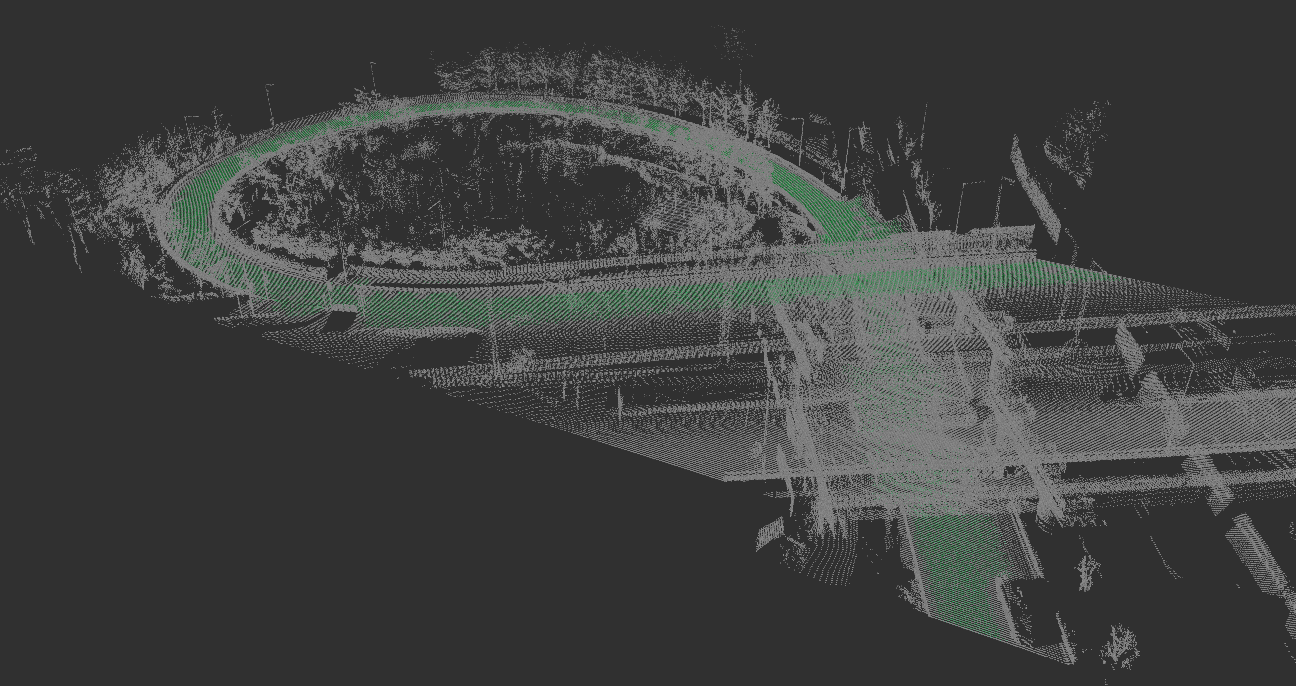
\includegraphics[width=\textwidth]{figures/map_bridge.png}
			\caption{Highway. Bridge with XY-overlap.}
			\label{fig:map_highway}
		\end{subfigure}
		\begin{subfigure}{0.32\textwidth}
			\centering
			
\includegraphics[width=\textwidth]{figures/map_crossing.png}
			\caption{Crossing. Cluttered.}
			\label{fig:map_crossing}
		\end{subfigure}
		\caption{Three complex outdoor environments.}
		\label{fig:maps}
	\end{figure*}
	
	\subsection{Scenario}
% TODO
%	\begin{itemize}
%		\item Description of the task.
%		\item Robot platform with dimensions and stats (it is only a prototype and not yet operational)
%		\item Figure of the robot
%		\item Description of the task execution
%		\item Description of the meta-CCP algorithm
%	\end{itemize}
	A road sweeper robot (Figure \ref{fig:robot}) of dimension $\text{length} = 1m$, $\text{breadth} = 0.75m$ and $\text{height} = 0.8m$ is tasked with cleaning the ground surface in an urban environment. The robot is assumed to travel at a slow enough speed to be safely avoidable by people (beside other safety measures in place). A comfortable walking speed is between 1.2 and 1.5 m/s for adults. The robot is assumed to travel a a speed of 1m/s. The robot actuators are most effective when the robot is traveling at a sufficiently slow speed, and more effective if the robot is driven straight than if it is rotating.
	
	A 3D point cloud of the target environment is available for offline CPP. In some cases there are stationary sensors, ground or areal 3D exploration has been performed earlier by other robots or the sweeper robot itself has previously scanned the environment. Local difference between the collected point cloud and what is observed when executing the coverage path is assumed to be neglectable due to the large scales involved. Any added locally-obstructive obstacles will in most cases have a minor effect on the overall cost of the coverage path.
	
	Given a point cloud and a starting point, traversible and coverable points are classified and collected using terrain assessment (\ref{sec:terrain-assessment}).\\
	\textbf{TODO}: Applying CPP algorithm. Domain adaptation with Parameter optimization.. Ok to use a lot of processing power (e.g. data center)..  Meta-algorithm?\\
	The resulting path is executed by a motion planner capable of collision avoidance \cite{krusi2017driving}. If the environment contains dynamic obstacles then a safe motion planner which can deal with dynamic obstacles is used \cite{andersson2018receding}.
	
	Due to the environment having complex border geometry is unreasonable to expect 100\% coverage of the actual coverable area. A planar or voxel-discretization approximation of only coverable cells would yield CCP solutions that are 100\% in the representation, but not necessarily to the real coverable geometry. As long as all traversible points reach 100\% coverage then it is acceptable that the coverage for coverable points to only get close to (but not reaching) 100\%.
			
	\begin{figure}
		\centering
		\begin{subfigure}{\columnwidth}
			\centering
			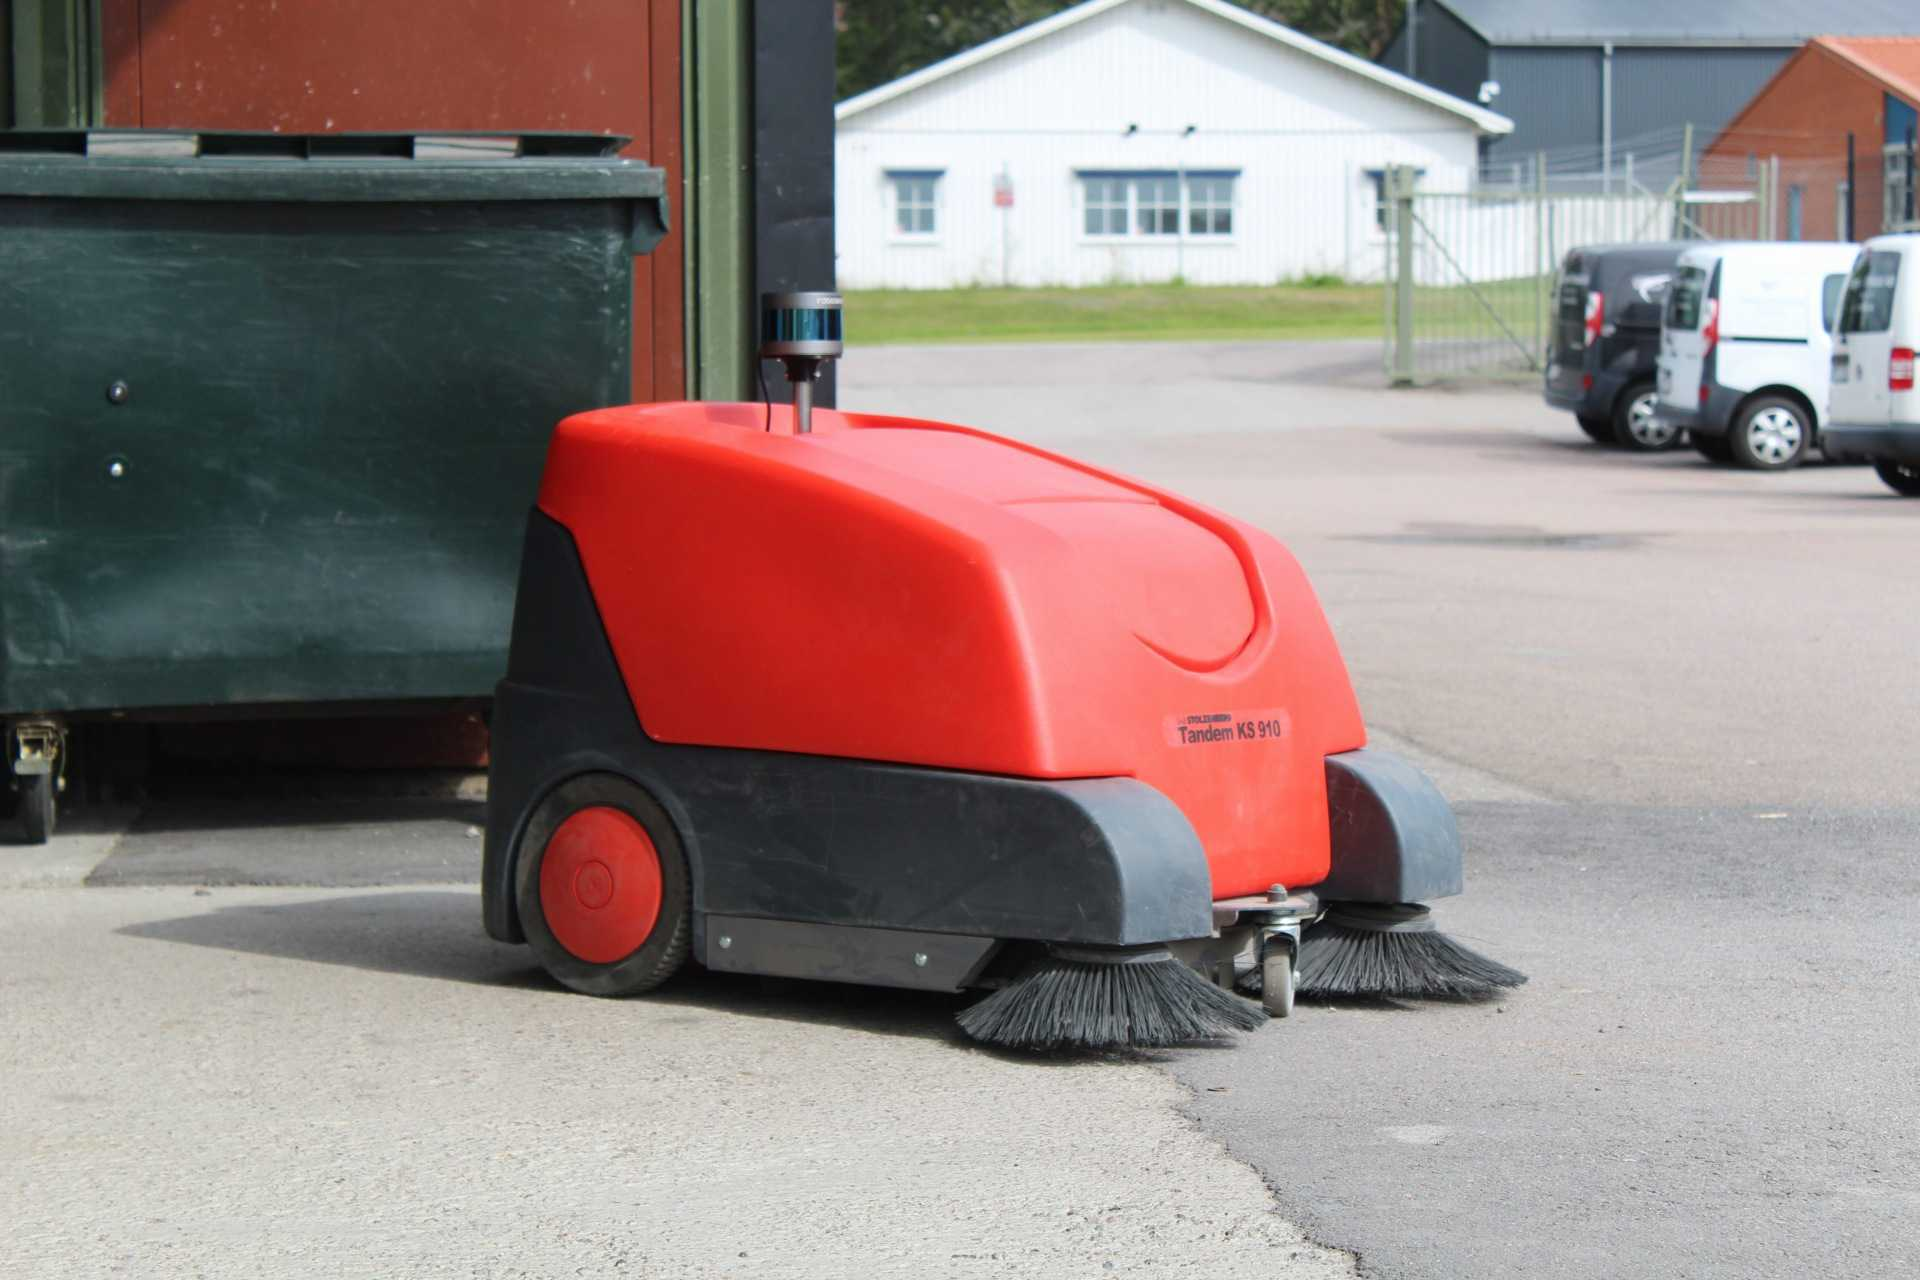
\includegraphics[width=\textwidth]{figures/sweeper_robot.jpg}
		\end{subfigure}
		\caption{The sweeper robot prototype, a modified Tandem KS 910 sweeping machine. }
		\label{fig:robot}
	\end{figure}
	
	
	
	\section{Evaluation}
	\label{sec:evaluation}
	
	Parameters for the Motion Planner are presented in Table \ref{tab:mp_parameters}.
	\begin{table}[h!]
		\centering
		\caption{Motion Planner parameter. Values of \emph{Resolution} parameters are set to give a good resolution while keeping the computational time on a reasonable level. \emph{Hand tuned based on tests} parameters are hand tuned by making multiple tests and adjust the values to give plausible reliance, computational time and paths.}
		\begin{tabular}{|l|c|l|c|}
			\hline 
			\textbf{Parameter} & \textbf{Value} & \textbf{Description} & \textbf{Based on} \\
			\hline 
			$\lambda$ & 0.1 m & Step size & Resolution \\
			$\lambda_{A*}$ & 0.5 m & Step size used in A* & Hand tuned b.o. tests \\
			$\lambda_{RRT}$ & 0.3 m & Step size used in RRT & Hand tuned b.o. tests \\
			$r_{trav}$ & 0.2 m & Threshold for untraversability & Hand tuned b.o. tests \\
			$N^{RRT}_{max}$ & 10 000 & Max iterations in RRT & Resolution \\
			\hline 
		\end{tabular}
		
		\label{tab:mp_parameters}
	\end{table}
	
	
	\subsection{Parameter Tuning}
	Time budget XYZ due to lower bound on area coverage by robot (traversible area divided by (robot footprint area times robot max speed)) being ABC hours.
	We use HyperOpt \cite{bergstra2013making} to search for the parameters that generate the best path for respective CPP algorithm. Parameters are sampled from the distributions in Table XYZ. HyperOpt use Adaptive Tree of Parzen Estimators \cite{bergstra2011algorithms} to estimate the next most likely parameter value to explore given the already explored parameter values. This makes HyperOpt much more efficient than for example random sampling. We ran 100 evaluations of HyperOpt for each algorithm, taking XYZ time.
	
	Parameters for the CPP algorithms are presented in Table \ref{tab:cpp_parameters} and Table \ref{tab:sampled_parameters}.
	\begin{table}[h!]
		\centering
		\caption{CPP Algorithms parameters. These values are calculated using the equations in Section \ref{sec:param_calc}.}
		\begin{tabular}{|l|l|c|}
			\hline 
			\textbf{Parameter} & \textbf{Description} & \textbf{Prior} \\
			\hline 
			$\lambda_{CPP}$ & Step size in CPP algoithms & $U(0.3,2)$\\
			$r_{visited}$ & Threshold for a position to be visited & $U(0.33,1)$\\
			\hline 
		\end{tabular}	
		\label{tab:cpp_parameters}
	\end{table}
	
	\begin{table}[h!]
		\centering
		\caption{Sampled BA* \& Inward Spiral parameters. These values are hand tuned by making multiple tests and adjusting the values to give good results regarding computational time, total rotation, length of path and coverage.}
		\begin{tabular}{|l|l|c|}
			\hline 
			\textbf{Parameter} & \textbf{Description} & \textbf{Prior} \\
			\hline 
			$r_{sampled}$ & Threshold for being visited & $U(\text{???})$ \\
			$N^{iter}_{max}$ & Max iterations of Sampled BA* paths & $U(30,200)$\\
			$N_{\phi}$ & Number of angles & $U(0.6,8.4)$\\
			$C_{1}$ & Coverage goal for Sampled BA* & $U(0.5,0.95)$\\
			$C_{2}$ & Total coverage goal & $U(\text{???})$\\
			$C_{min}$ & Min. coverage for a BA* segment & $U(0.001,0.05)$\\
			$N_{min}$ & Min. \#points in Inward Spiral segment & $U(2,100)$\\
			\hline 
		\end{tabular}	
		\label{tab:sampled_parameters}
	\end{table}
	
	\begin{table}[h!]
		\centering
		\caption{Used parameters values (found using HyperOpt).}	
		\begin{subfigure}{.4\columnwidth}
			%\centering
			\caption{Method 1}\vspace{-0.5em}
			\begin{tabular}{|l|l|}
				\hline 
				\textbf{Parameter} & \textbf{Value} \\	
				\hline 
				$\lambda_{CPP}$ & $\text{???}$\\
				$r_{visited}$ & $\text{???}$\\
				\hline 
			\end{tabular}
		\end{subfigure}
		~
		\begin{subfigure}{.4\columnwidth}
			%\centering
			\caption{Method 2}\vspace{-0.5em}
			\begin{tabular}{|l|l|}
				\hline 
				\textbf{Parameter} & \textbf{Value} \\	
				\hline 
				$\lambda_{CPP}$ & $\text{???}$\\
				$r_{visited}$ & $\text{???}$\\
				\hline 
			\end{tabular}
		\end{subfigure}\vspace{1em}
		\\
		\begin{subfigure}{.4\columnwidth}
			%\centering
			\caption{Method 3}\vspace{-0.5em}
			\begin{tabular}{|l|l|}
				\hline 
				\textbf{Parameter} & \textbf{Value} \\	
				\hline 
				$\lambda_{CPP}$ & $\text{???}$\\
				$r_{visited}$ & $\text{???}$\\
				\hline 
			\end{tabular}
		\end{subfigure}
		~
		\begin{subfigure}{.4\columnwidth}
			%\centering
			\caption{Method 4}\vspace{-0.5em}
			\begin{tabular}{|l|l|}
				\hline 
				\textbf{Parameter} & \textbf{Value} \\	
				\hline 
				$\lambda_{CPP}$ & $\text{???}$\\
				$r_{visited}$ & $\text{???}$\\
				\hline 
			\end{tabular}	
		\end{subfigure}\vspace{1em}
		\\
		\begin{subfigure}{.4\columnwidth}
			%\centering
			\caption{Method 5}\vspace{-0.5em}
			\begin{tabular}{|l|l|}
				\hline 
				\textbf{Parameter} & \textbf{Value} \\
				\hline 
				$r_{sampled}$ & $\text{???}$ \\
				$N^{iter}_{max}$ & $\text{???}$\\
				$N_{\phi}$ & $\text{???}$\\
				$C_{1}$ & $\text{???}$\\
				$C_{2}$ & $\text{???}$\\
				$C_{min}$ & $\text{???}$\\
				$N_{min}$ & $\text{???}$\\
				\hline 
			\end{tabular}	
		\end{subfigure}
		\label{tab:best_parameters}
	\end{table}
	
	%\section{Experiment 1 - BA*, Inward Spiral and Curved BA* over Time}
	%Results of Experiment 1 is presented in the Figures \ref{fig:exp1_coverage}-\ref{fig:exp1_rotation}. 
	%
	%\begin{figure}
	%	\centering
	%	\begin{subfigure}{0.85\columnwidth}
	%		\centering
	%		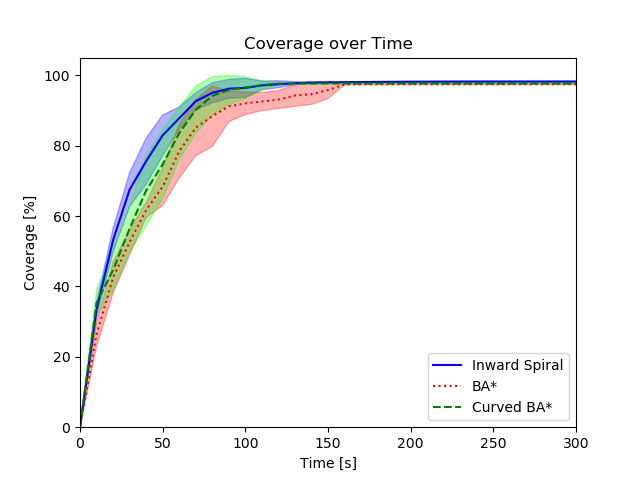
\includegraphics[width=\textwidth]{figures/exp1_coverage.png}
	%		\caption{Full view.}
	%		\label{fig:exp1_coverage_full}
	%	\end{subfigure}
	%	\begin{subfigure}{0.85\columnwidth}
	%		\centering
	%		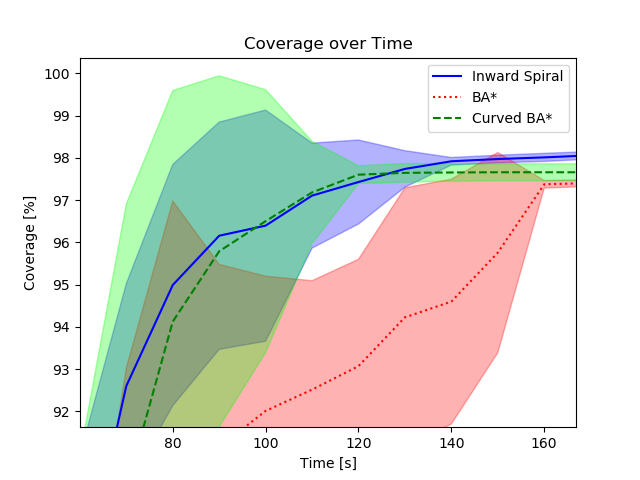
\includegraphics[width=\textwidth]{figures/exp1_coverage_zoom.png}
	%		\caption{Zoomed in view.}
	%		\label{fig:exp1_coverage_zoom}
	%	\end{subfigure}
	%	\caption{Results of Experiment 1. Means and standard deviations of coverage over time.}
	%	\label{fig:exp1_coverage}
	%\end{figure}
	%
	%\begin{figure}
	%	\centering
	%	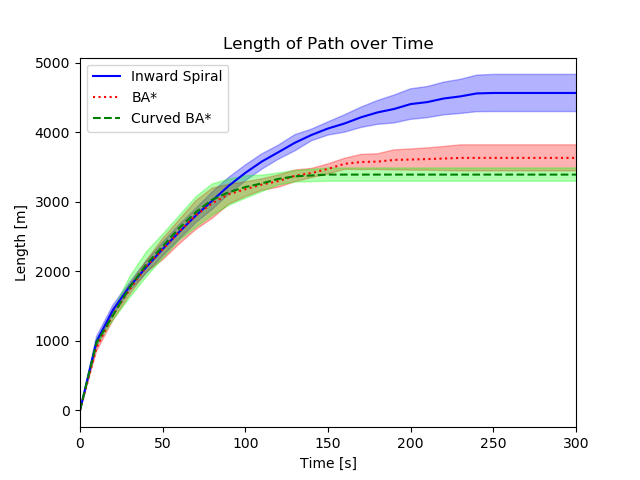
\includegraphics[width=0.85\columnwidth]{figures/exp1_length.png}
	%	\caption{Results of Experiment 1. Means and standard deviations of path length over time.}
	%	\label{fig:exp1_length}
	%\end{figure}
	%
	%
	%\begin{figure}
	%	\centering
	%	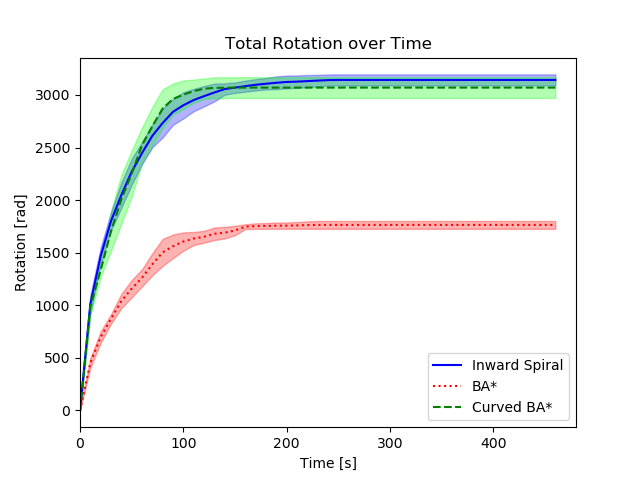
\includegraphics[width=0.85\columnwidth]{figures/exp1_rotation.png}
	%	\caption{Results of Experiment 1. Means and standard deviations of rotation over time.}
	%	\label{fig:exp1_rotation}
	%\end{figure}
	
	
	%\section{Experiment 2 - Tuning of $d_{max}$ for Sampled BA* \& Inward Spiral}
	%Results of Experiment 2 is presented in the Figures \ref{fig:exp2_time}-\ref{fig:exp2_rotation}. The average coverage for all paths in Experiment 2 was 98.3\%. To be able to compare with the algorithms in Experiment 1, their means and standard deviations for computational time, path length and total rotation at 98.3\% from Experiment 1 are shown in the figures as well.
	%
	%\begin{figure}
	%	\centering
	%	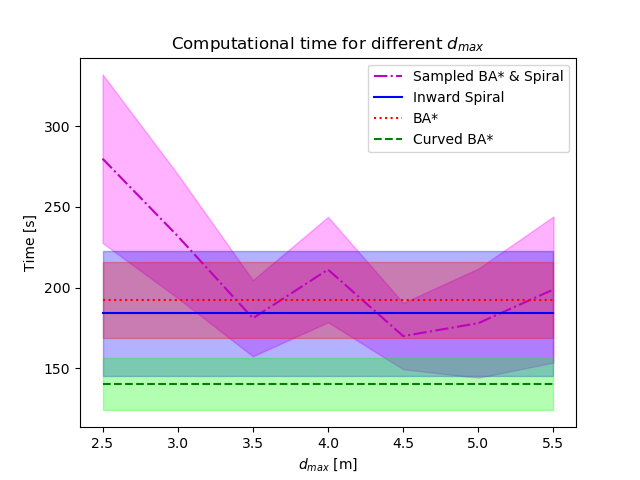
\includegraphics[width=0.85\columnwidth]{figures/exp2_time.png}
	%	\caption{Results of Experiment 2. Means and standard deviations of computational time for different values of parameter $d_{max}$ for Sampled BA* \& Inward Spiral. Means and standard deviations for computational time in Experiment 1 at 98.3\% are shown in the figure as well.}
	%	\label{fig:exp2_time}
	%\end{figure}
	%
	%\begin{figure}
	%	\centering
	%	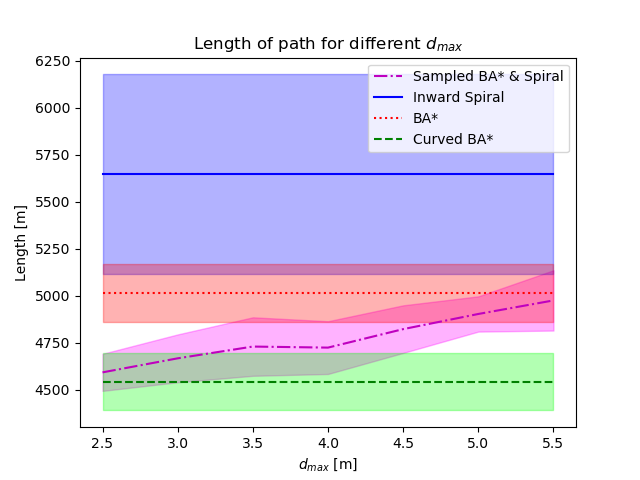
\includegraphics[width=0.85\columnwidth]{figures/exp2_length.png}
	%	\caption{Results of Experiment 2. Means and standard deviations of path length for different values of parameter $d_{max}$ for Sampled BA* \& Inward Spiral. Means and standard deviations for path length in Experiment 1 at 98.3\% are shown in the figure as well.}
	%	\label{fig:exp2_length}
	%\end{figure}
	%
	%\begin{figure}
	%	\centering
	%	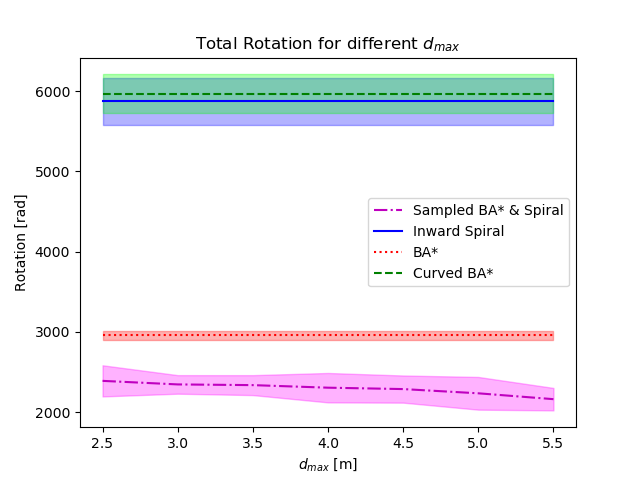
\includegraphics[width=0.85\columnwidth]{figures/exp2_rotation.png}
	%	\caption{Results of Experiment 2. Means and standard deviations of total rotation for different values of parameter $d_{max}$ for Sampled BA* \& Inward Spiral. Means and standard deviations for total rotation in Experiment 1 at 98.3\% are shown in the figure as well.}
	%	\label{fig:exp2_rotation}
	%\end{figure}
	
	\subsection{Coverage Path Planning}
	
	\begin{figure}
		\centering
		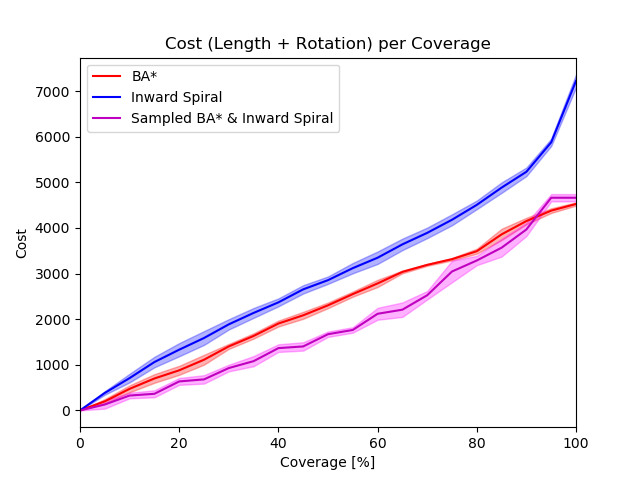
\includegraphics[width=\columnwidth]{figures/garage_pre_restult_coverage.png}
		\caption{Path cost vs coverage on the Garage environment.}
		\label{fig:result-garage-cost-coverage}
	\end{figure}
	
	\begin{figure}
		\centering
		\begin{subfigure}{0.48\columnwidth}
			\centering
			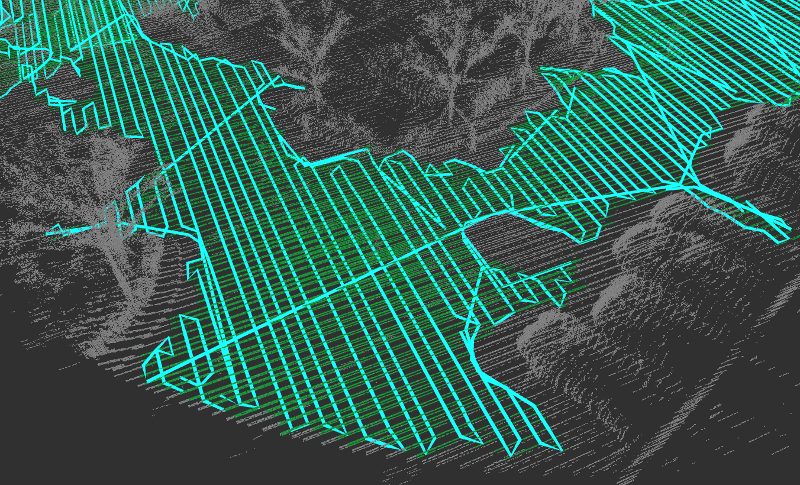
\includegraphics[width=\textwidth]{figures/example_bastar2.png}
			\caption{BA*}
			\label{fig:example_bstar}
		\end{subfigure}
		\begin{subfigure}{0.48\columnwidth}
			\centering
			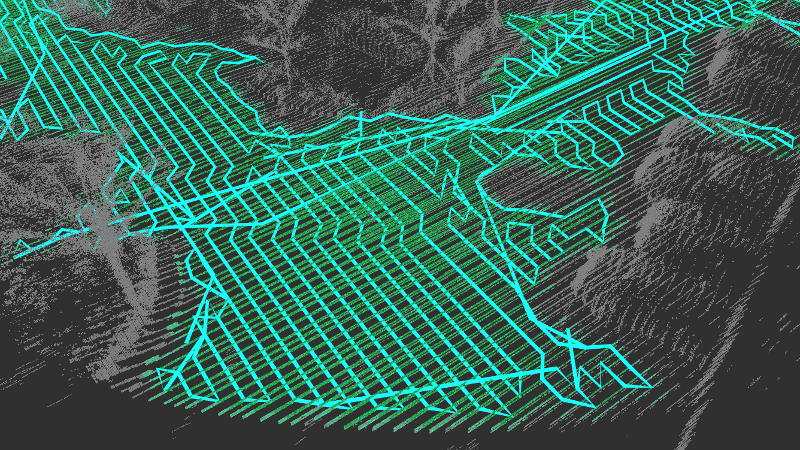
\includegraphics[width=\textwidth]{figures/example_curved_bastar.png}
			\caption{Curved BA*}
			\label{fig:example_curved_bstar}
		\end{subfigure}
		\\
		\begin{subfigure}{0.48\columnwidth}
			\centering
			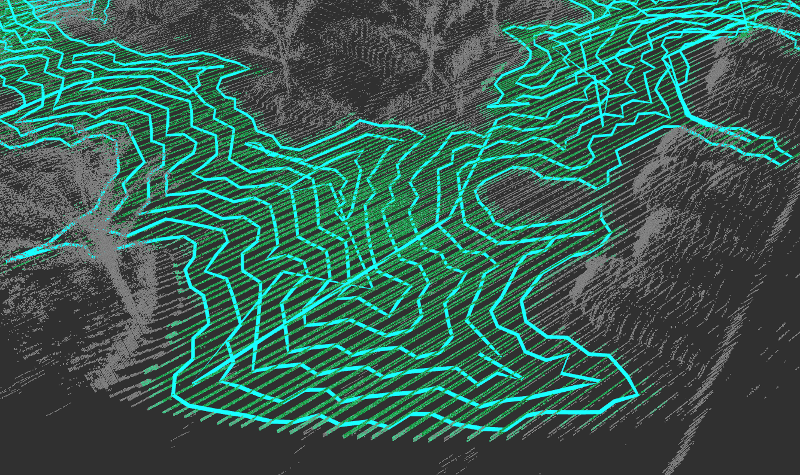
\includegraphics[width=\textwidth]{figures/example_inward_spiral.png}
			\caption{Inward Spiral}
			\label{fig:example_inward_spiral}
		\end{subfigure}
		\begin{subfigure}{0.48\columnwidth}
			\centering
			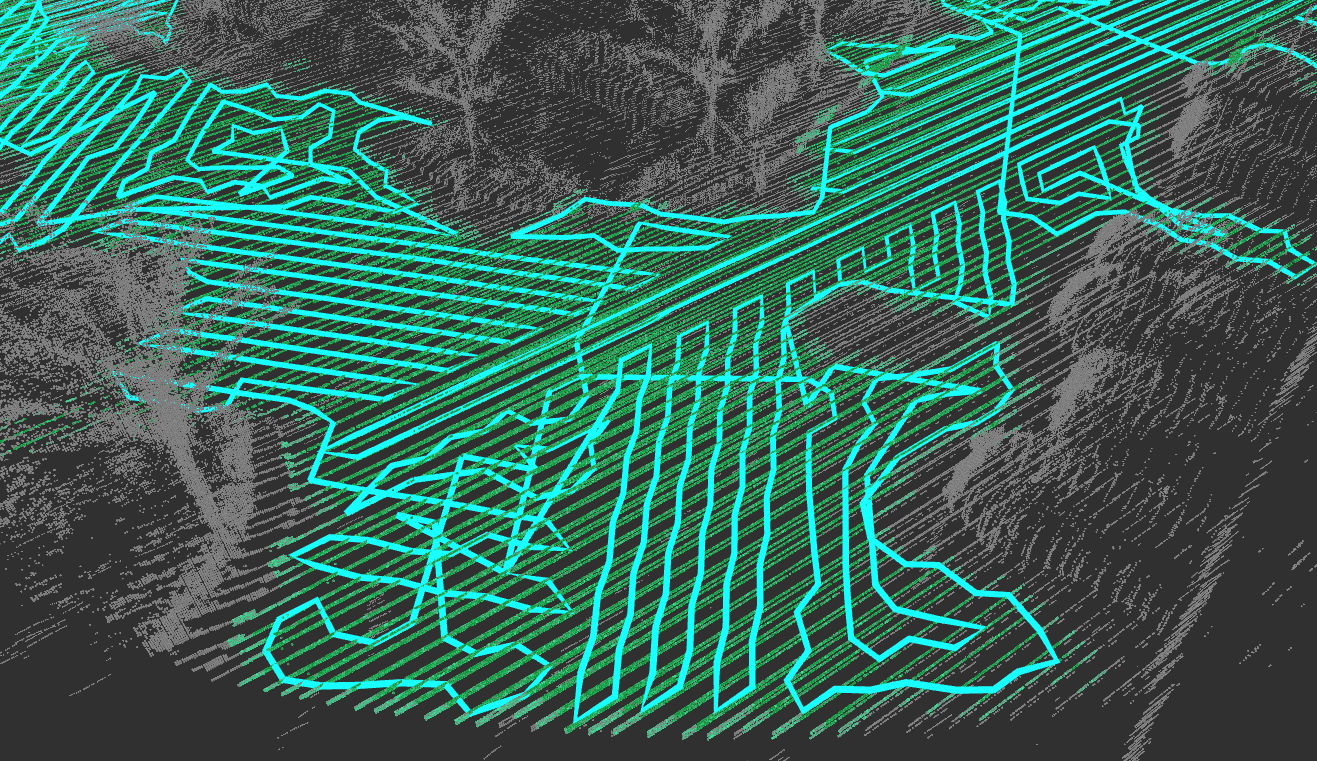
\includegraphics[width=\textwidth]{figures/example_sampled_bastar.png}
			\caption{Sampled BA*}
			\label{fig:example_sampled_bstar}
		\end{subfigure}
		\caption{}
		\label{fig:algorithm_experiment_examples}
	\end{figure}
	
	
	\section{Conclusions}
	\label{sec:conclusions}
	\begin{itemize}
		\item Compare with learning-based methods: A* search and learned heuristic.
		\item Future work: Real experiments in varied garage maps when sweeper robot prototype is operational.
	\end{itemize}
	
	%%%%%%%%%%%%%%%%%%%%%%%%%%%%%%%%%%%%%%%%%%%%%%%%%%%%%%%%%%%%%%%%%%%%%%%%%%%%%%%%
	%\section*{APPENDIX}
	
	
	%\section*{ACKNOWLEDGMENT}
	%
	%The preferred spelling of the word �acknowledgment� in America is without an �e� after the �g�. Avoid the stilted expression, �One of us (R. B. G.) thanks . . .�  Instead, try �R. B. G. thanks�. Put sponsor acknowledgments in the unnumbered footnote on the first page.
	
	
	
	%%%%%%%%%%%%%%%%%%%%%%%%%%%%%%%%%%%%%%%%%%%%%%%%%%%%%%%%%%%%%%%%%%%%%%%%%%%%%%%%
	
	\bibliographystyle{IEEEtran}
	\bibliography{bibliography}
	
	
	
\end{document}
